\documentclass[a4paper, 
amsfonts, 
amssymb, 
amsmath, 
reprint, 
showkeys, 
nofootinbib, 
twoside]{revtex4-2}
\usepackage[english]{babel}
\usepackage[utf8]{inputenc}
\usepackage[pdftex, pdftitle={Article}, pdfauthor={Author}, hidelinks]{hyperref} % For hyperlinks in the PDF
\usepackage{xcolor}
\usepackage{bm}
\usepackage{physics}
\usepackage{graphicx}
\DeclareMathAlphabet{\mymathbb}{U}{BOONDOX-ds}{m}{n} % Fancy E for Exp value 
%\setlength{\marginparwidth}{2.5cm}


\bibliographystyle{apsrev4-1} 

\begin{document}
\title{ Linear Regression, Resampling and Machine Learning \\
FYS-STK4155 Project 1}

\author{Halvor Melkild}
    \email[Correspondence email address: ]{halvor.melkild@fys.uio.no}
    \affiliation{Department of Physics, University of Oslo}

\author{Martin Tømterud}
    \email[Correspondence email address: ]{martin.tomterud@uib.no}
    \affiliation{Department of Physics and Technology, University of Bergen}
    \affiliation{Centre for Materials Science and Nanotechnology, University of Oslo}

\author{\textcolor{blue}{\href{https://github.com/martintomterud/DA-ML}{Code available at git rep https://github.com/martintomterud/DA-ML}}} 

\date{\today} 

\begin{abstract}
Different methods of linear regression are compared on two datasets; one generated by the Franke function and one set of topographical data. We find that ordinary least squares regression gives the lowest mean square error, outperforming the more complex ridge and lasso regression methods. We postulate that this is due to the complexity of the data we analyse, which prevents overfitting using OLS, making the advantages of ridge and lasso unimportant for the present data.
\end{abstract}

\keywords{machine learning, ridge regression, lasso regression, bootstrap resampling, cross validation}

\maketitle


\section{Introduction}

As larger and larger datasets are produced by scientists, the use of ``classical'' statistical methods have been debated in the community. Particularly, there has been an increasing interest in developing efficient statistical tools for the analysis of large amounts of data. Machine learning is a technique that has generated interest and enthusiasm from scientists in all fields. The collection of techniques available is rapidly growing, all from simple linear regression to unsupervised learning. In the case of supervised learning techniques, which include linear regression, the goal is to extract a model relating the in- and output, from a set of known cases. 

In this paper we analyse and compare three different methods of linear regression. These are Ordinary Least Squares, Ridge regression and Lasso regression. In Section~\ref{theory} we introduce the concept of linear regression and the details of the three methods we want to compare. The resampling techniques, used for testing the methods, are discussed in Section~\ref{methods}. The results are presented in Section~\ref{results} and here we also discuss our findings. We explore the relationship between the bias and variance of the models in each of the three cases. The methods are tested on two different datasets; the first set is generated by the analytic Franke function and the second is generated by real world terrain data.


\section{Theory}
\label{theory}

We begin by introducing the general ideas behind linear regression. Then follows a presentation of the three different implementations we are testing. We also show how the bias and variance contributes to the expected error of our models. 


\subsection{Linear Regression}
Suppose we have a sample of $n$ observed outcomes, $y_i$, where the features of the input is assumed to be characterised by $m$ variables. The set of values of these variables for each sample is organised in the $n\times m$ design matrix, $\bm{X}$. The set of observations is called the response, and is a vector of length $n$;
\begin{equation}
    \bm{y} = [y_1, \: y_2,\: \dots, \: y_n].
\end{equation}
In general, each element of both $\bm{X}$ and $\bm{y}$ can be multi-dimensional variables, but for our use, they will simply be scalar variables. Finding relevant input variables to construct the design matrix, is one of the main challenges when building a regression model. Both for the Franke function and the topological data, we are considering a continuous map from two dimensions to one. The output $y_i$ could therefore be approximated by a polynomial in the two coordinates, $x_{1i}$ and $x_{2i}$. Our design matrix is therefore chosen as
\begin{equation}
    X = \begin{pmatrix} 
            1 & x_{11} & x_{21} & x_{11}x_{21} & x_{11}^2 & x_{21}^2 & \cdots & x_{21}^p\\ 
            1 & x_{12} & x_{22} & x_{12}x_{22} & x_{12}^2 & x_{22}^2 & \cdots & x_{22}^p\\
            \vdots & \vdots & \vdots & \vdots & \vdots & \vdots &  \ddots & \vdots \\
            1 & x_{1n} & x_{2n} & x_{1n}x_{2n} & x_{1n}^2 & x_{2n}^2 & \cdots & x_{2n}^p
        \end{pmatrix},
\end{equation}
where the number of columns, $m$, is decided by the polynomial degree, $p$, we want to work with
\begin{equation}
    m = \frac{1}{2}(p+1)(p+2).
\end{equation}

The aim with regression is to find a model which explains the response, $\bm{y}$, in terms of the quantities in $\bm{X}$. A good model should be able to predict $y$ for future events, with satisfying precision. We will assume that $\bm{y}$ can be understood in terms of a continuous function $f(\bm{X})$ and some noise or error, $\bm{\epsilon}$, on the form
\begin{equation}
    \bm{y} = f(\bm{X}) + \bm{\epsilon}.
    \label{eq:y_f}
\end{equation}
The noise will throughout be assumed to follow a normal distribution with mean $\mu = 0$, and variance $\mathrm{Var}(\epsilon) = \sigma^2$.

In the present work, we will focus on \textit{linear} regression, \textit{i.e.} we will assume that $f$ depends linearly on $X$, 
\begin{equation}
    \bm{y} = \bm{X}\bm{\beta} + \bm{\epsilon}.
    \label{eq:yXbe}
\end{equation}
The vector $\bm{\epsilon}$ is the deviation from the linear response model, which is given by $\bm{X}\bm{\beta}$, where $\bm{\beta}$ is the vector containing the linear regression coefficients. We denote our linear model as,
\begin{equation}
    \bm{\tilde{y} = \bm{X}\bm{\beta}}.
\end{equation} 
The error made by the linear model can therefore be expressed as
\begin{equation}
    \bm{\epsilon} = \bm{y} - \bm{\tilde{y}}.
\end{equation}
The objective of our regression analysis is to determine $\bm{\beta}$ in such a way that the linear model matches the data in the ``best'' possible way. To define what we mean by ``best'', we have to introduce a measure, called the \textit{cost} function, $C(\bm{\beta})$. In general, the cost function should be a measure of the size of $\bm{\epsilon}$ and the optimal $\bm{\beta}$ should minimise $C$. The definition of the cost function another of the challenge when building a regression model, where the choice heavily influences the final outcome. Depending on the dataset and selected model, different definitions of $C$ might be more or less suitable. The definition of the cost function is what separates the three different methods we will study, ordinary least squares (OLS), ridge and lasso regression.


\subsection{Ordinary Least Squares}

The OLS method is discussed for instance in Hastie, Tibshirani, and Friedman~\cite[Chapter 2]{Hastie}, and we follow the discussion presented there. 

The method imposes the standard Euclidean $L^2$-norm on the vector space, and defines the cost function simply as the squared norm of the error vector,
\begin{align}
\begin{split}
    C^\textrm{OLS}(\bm{\beta}) &= \lVert \bm{\epsilon} \rVert^2 \\
    &= \lVert \bm{y} - \bm{\tilde{y}} \rVert^2 \\
\end{split}
\end{align}
This is equivalent to the mean square error (MSE), 
\begin{equation}
    \textrm{MSE}(\bm{y}, \bm{\tilde{y}}) = \frac{1}{n}\sum_{i = 1}^n (y_i - \tilde{y}_i)^2.
\end{equation}
On vector form we therefore define our cost function as
\begin{equation}
    C^{\textrm{OLS}}(\bm{\beta}) = \frac{1}{n}(\bm{y} - \bm{X\beta})^T(\bm{y} - \bm{X\beta}).
\end{equation}

We find the optimal value of $\bm{\beta}^{\textrm{OLS}}$ by differentiating $C$ by $\beta$ and equating the result to zero:
\begin{equation}
    \frac{\partial C^{\textrm{OLS}}(\bm{\beta})}{\partial \bm{\beta}} = -\frac{2}{n}\bm{X}^T(\bm{y} - \bm{X\beta})
\end{equation}
\begin{equation}
    \Rightarrow 0 = \bm{X}^T(\bm{y} - \bm{X}\bm{\beta}^{\textrm{OLS}})
\end{equation}
\begin{equation}
    \Rightarrow \bm{\beta}^{\textrm{OLS}} = (\bm{X}^T\bm{X})^{-1}\bm{X}^T\bm{y}
    \label{eq:betaOLS}
\end{equation}
The predicted output, $\bm{\tilde{y}}$, is now obtained from the input $\bm{X}$, and output $\bm{y}$
\begin{equation}
    \bm{\tilde{y}} = \bm{X\beta}^{\textrm{OLS}} = \bm{X}(\bm{X}^T\bm{X})^{-1}\bm{X}^T\bm{y}
\end{equation}

From Eq.~\eqref{eq:betaOLS} we can derive the variation in $\bm{\beta}^\textrm{OLS}$.
\begin{align}
\begin{split}
    \textrm{Var}(\bm{\beta}^{\textrm{OLS}}) 
        &= \mathbb{E}[\bm{\beta}_\textrm{OLS} \bm{\beta}_\textrm{OLS}^T] 
            - \mathbb{E}[\bm{\beta}_\textrm{OLS}]\mathbb{E}[\bm{\beta}_\textrm{OLS}^T] \\
        &= (\bm{X}^T\bm{X})^{-1}\bm{X}^T \\
        &\qquad \times (\mathbb{E}[\bm{y}\bm{y}^T] - \mathbb{E}[\bm{y}]\mathbb{E}[\bm{y}]^T) \\
        &\qquad \times \bm{X} (\bm{X}^T \bm{X})^{-1} \\
        &= (\bm{X}^T\bm{X})^{-1}\bm{X}^T \textrm{Var}(\bm{y}) \bm{X} (\bm{X}^T \bm{X})^{-1}.
\end{split}
\label{eq:varbeta}
\end{align}
From our assumption of the form of $\bm{y}$ in Eq.~\eqref{eq:yXbe} and the normal distribution of $\bm{\epsilon}$, it follows that 
\begin{equation}
    \mathbb{E}[\bm{y}] = \mathbb{E}[\bm{X}\bm{\beta}] + \mathbb{E}[\bm{\epsilon}] = \bm{X}\bm{\beta}
\end{equation}
and 
\begin{align}
    \mathbb{E}[\bm{y}\bm{y}^T] 
        = \bm{X}\bm{\beta} \bm{\beta}^T \bm{X}^T + \sigma^2 \bm{I}.
\end{align}
This gives us 
\begin{equation}
    \textrm{Var}(\bm{y}) = \sigma^2 \bm{I},
\end{equation}
which we can insert in Eq.~\eqref{eq:varbeta} and conclude that
\begin{equation}
    \textrm{Var}(\bm{\beta}) = (\bm{X}^T\bm{X})^{-1} \sigma^2.
\end{equation}


\subsection{Ridge Regression}

The approach for finding $\beta$ with Ordinary Least Squares demand that $\bm{X}^T \bm{X}$ is invertible. If not, $\beta^\textrm{OLS}$ is not uniquely defined. To avoid this problem, we can introduce a positive regularisation parameter $\lambda$
\begin{equation}
    \bm{X}^T\bm{X} \to \bm{X}^T\bm{X} + \lambda \bm{I}.
\end{equation}
making sure the matrix is invertible. This is equivalent to modifying the cost function to the one that defines ridge regression, \cite{Hoerl}
\begin{align}
\begin{split}
        C^{\textrm{R}}(\bm{\beta}) &= \lVert \bm{y} - \bm{\tilde{y}}\rVert^2 + \lambda \lVert \bm{\beta}\rVert^2 \\
        &= (\bm{y} - \bm{X\beta})^T(\bm{y} - \bm{X\beta}) + \lambda \bm{\beta}^T \bm{\beta}.
\end{split}
\label{eq:ridgecost}
\end{align}
Again, taking the derivative with respect to $\bm{\beta}$ and equating to zero gives the optimal value, $\bm{\beta}^{\textrm{R}}$, for the Ridge regression method,
\begin{equation}
   \frac{\partial C^{\textrm{R}}(\bm{\beta})}{\partial \bm{\beta}} = -2\bm{X}^T(\bm{y} - \bm{X\beta}) + 2 \lambda \bm{I} \bm{ \beta} 
\end{equation}
\begin{equation}
    \Rightarrow \bm{\beta}^{\textrm{R}} = (\bm{X}^T\bm{X} + \lambda\bm{I})^{-1}\bm{X}^T\bm{y}.
\end{equation}
We observe that in the limit $\lambda = 0$, Ridge regression reduces to OLS.

From the cost function we notice that $\lambda$ penalises bigger $\bm{\beta}$'s. It's effect is therefore to shrink the all the components of $\bm{\beta}^{\textrm{R}}$, but equally. Doing a \textit{singular value decomposition} of $\bm{X}$, one finds that the directions in the column space of $\bm{X}$ with the smallest variance shrinks the most. As a consequence, the method does not treat all input parameters as equally important, but the main weight is put on those with higher variance. Under the assumption that the directions with low variance are of less importance, ridge regression therefore helps with reducing the effective degrees of freedom in the problem and could reduce the share of the variance in $\beta$ which comes from the directions we deem less important.


\subsection{Lasso Regression}
Lasso regression differs from Ridge regression in the metric imposed on $\bm{\beta}$ in the shrinking term. Instead of using the $L^2$ norm we instead impose the $L^1$ norm on the shrinkage term only, so that the cost function reads
\begin{align}
\begin{split}
        C^{\textrm{L}}(\bm{\beta}) &= \lVert \bm{y} - \bm{\tilde{y}}\rVert^2 + \lambda \lVert \bm{\beta}\rVert \\
        &= (\bm{y} - \bm{X\beta})^T(\bm{y} - \bm{X\beta}) + \lambda \lvert \bm{\beta} \rvert.
\end{split}
\end{align}
There is no explicit analytical derivation for a $\bm{\beta}$ that minimises $C^{\textrm{L}}(\bm{\beta})$ like there is for Ridge and OLS. Instead numerical methods like gradient descent is employed to find the optimal value of $\bm{\beta}$.

\subsection{Statistical Metrics}

To measure the error and performance of our models we employ statistical metrics that can measure the errors made by the methods and compare their performance. 
One such tool has already been introduced, the mean square error, which reads
\begin{equation}
    \textrm{MSE}(\bm{y}, \bm{\tilde{y}}) = \frac{1}{n}\sum_{i = 1}^n (y_i - \tilde{y}_i)^2.
\end{equation}
Another useful metric is the $R^2$-score, also known as the coefficient of determination, which measures to what extent the variation in $\bm{y}$ is explained by the model $\bm{\tilde{y}}$. The $R^2$-score reads
\begin{equation}
    \textrm{R}^2(\bm{y}, \bm{\tilde{y}}) = 1 - \frac{\sum_{i = 1}^n (y_i - \tilde{y}_i)^2}{\sum_{i = 1}^n (y_i - \bar{y}_i)^2},
\end{equation}
where we have introduced the mean
\begin{equation}
    \bar{y} = \frac{1}{n}\sum_{i = 1}^n y_i.
\end{equation}

\subsection{Bias-Variance}

The bias and the variance of the predictions of the regression algorithms are related to the MSE, or the cost function, that we use as a criterion to optimise our $\bm{\beta}$-parameter.  
The variance of the resulting MSE quantifies how the prediction is expected to change if the model is trained on a different set of training data. A good model therefore should have a low variance and it should retain a low variance as the training set is altered. Flexible models are known to produce larger variances and the predictions can therefore vary more. 
The bias quantifies the error that is made by imposing a relation between the response $\bm{y}$ and the known quantities $\bm{X}$. In this work we assume a linear relation between the two, and the bias therefore quantifies the error made by the linear relationship,  or alternatively, how non-linear the response is.
Knowing that the expected value $\mathbb{E}$ is equal to the MSE, 
\begin{equation}
    \mathbb{E}\left[(\mathbf{y} - \mathbf{\tilde{y}})^2\right] = \frac{1}{n}\sum_{i = 0}^{n-1} (y_i - \tilde{y}_i)^2,
\end{equation}
we can derive that the relation between the MSE, bias and variance is
\begin{align}
\label{eq:bivar}
    \begin{split}
        \mathbb{E}\left[(\mathbf{y} - \mathbf{\tilde{y}})^2\right] &= \frac{1}{n}\sum_{i = 0}^{n-1} (f_i - \mathbb{E}[\tilde{y}_i])^2 \\
        &+ \frac{1}{n}\sum_{i = 0}^{n-1} (\tilde{y}_i - \mathbb{E}[\tilde{y}_i])^2 \\
        &+ \sigma^2 \\
        &= \mathrm{Bias}^2 + \mathrm{Variance} + \sigma^2.
    \end{split}
\end{align}
In the above we have used $f_i = y_i - \epsilon_i$, by rewriting Eq.~\eqref{eq:y_f} on component form. This equation therefore tells us that to lower the MSE we want a low bias and a low variance. The $\sigma^2$-term arises from the normal distribution of the error, $\epsilon$. This is referred to as an irreducible error in the literature.

We would ultimately like to choose the regression model that gives a MSE as low as possible, and by Eq.~\eqref{eq:bivar} this would imply choosing a model with low bias and low variance. However, as just discussed, improving the flexibility of a model is often associated with improving the bias, but giving a higher variance. This is called the bias-variance trade-off, and implies that one often has to look for some compromise. 

We use the following relations in the proof of Eq.~\eqref{eq:bivar} below.
\begin{equation}
	\mathbb{E}[X^2] = \mathrm{Var}[X] + \left(\mathbb{E}[X]\right)^2
\end{equation}
\begin{equation}
	\mathbb{E}[f]=f \Rightarrow \mathbb{E}[y]=\mathbb{E}[f+\epsilon] = f
\end{equation}
\begin{equation}
	\mathrm{Var}[\epsilon] = \sigma^2 \Rightarrow \mathrm{Var}[y] = \mathbb{E}[(f+\epsilon-f)^2] = \sigma^2
\end{equation}
\begin{align}\label{eq:der_bivar}
\begin{split}
	\mathbb{E}[(y-\tilde{y})^2] =& \mathbb{E}[(f+\epsilon - \tilde{y})^2] \\
	=& \mathbb{E}[\left(f+\epsilon - \tilde{y} + \mathbb{E}[\tilde{y}] - \mathbb{E}[\tilde{y}]\right)^2] \\
	=& \mathbb{E}[(f-\mathbb{E}[\tilde{y}])^2] + \mathbb{E}[\epsilon^2] + \mathbb{E}[(\mathbb{E}[\tilde{y}]-\tilde{y})^2] \\
	&+ 2\mathbb{E}[(f-\mathbb{E}[\tilde{y}])\epsilon] 
	+ 2\mathbb{E}[\epsilon(\mathbb{E}[\tilde{y}]-\tilde{y})] \\ &+ 2\mathbb{E}[(\mathbb{E}[\tilde{y}]-\tilde{y})(f-\mathbb{E}[\tilde{y}])] \\
	=& (f-\mathbb{E}[\tilde{y}])^2 + \mathbb{E}[\epsilon^2] + \mathbb{E}[(\mathbb{E}[\tilde{y}]-f)^2] \\
	&+ 2(f-\mathbb{E}[\tilde{y}])\mathbb{E}[\epsilon] 
	+ 2\mathbb{E}[\epsilon]\mathbb{E}[\mathbb{E}[\tilde{y}]-\tilde{y}] \\ &+ 2\mathbb{E}[\mathbb{E}[\tilde{y}]-\tilde{y}](f-\mathbb{E}[\tilde{y}]) \\
	=& (f-\mathbb{E}[\tilde{y}])^2 + \mathbb{E}[(\mathbb{E}[\tilde{y}]-\tilde{y})^2] + \mathbb{E}[\epsilon^2]  \\
	=& \mathrm{Bias}[\tilde{y}]^2  + \mathrm{Var}[\tilde{y}] + \sigma^2
\end{split}
\end{align}

\subsection{The Franke Function}
For $x,y \in [0, 1]$, the Franke function is given by~\cite{Franke}
\begin{align}\label{eq:franke}
\begin{split}
	f\left(x,y\right) &=\frac{3}{4}\exp\left(-\frac{\left(9x-2\right)^2}{4}-\frac{\left(9y-2\right)^2}{4} \right) \\
	&+\frac{3}{4}\exp\left(-\frac{\left(9x+1\right)^2}{49}-\frac{\left(9y+1\right)^2}{10} \right) \\
	&+\frac{1}{2}\exp\left(-\frac{\left(9x-7\right)^2}{4}-\frac{\left(9y-3\right)^2}{4} \right) \\
	&-\frac{1}{5}\exp\left(-\left(9x-4\right)^2-\left(9y-7\right)^2 \right).
	\end{split}
\end{align}

\section{Methods}
\label{methods}

We apply two different resampling methods in the present project to test the validity of our model by computing predictions on randomly selected subsets of our data. 

\subsection{Bootstrap Resampling}
With bootstrap resampling, the approach is to compute averages of several small data samples that are drawn from the main training set and then replaced. We then compute the regular statistics on the smaller data sets and compute the averages of all the smaller data set statistics. The bootstrap is particularly useful for evaluating bias and variance, and we use it to investigate the bias variance crossover in our model, to determine at which complexity the linear model breaks down and where we obtain the lowest MSE.

\subsection{$k$-fold Cross Validation}

Cross validation is a method for evaluating the performance of a machine learning model. We split the total dataset into $k$ folds (or groups), and retain one as a testing set, while we use the rest as a training set. After fitting the model to the training set, we evaluate it on the test set and compute the evaluation scores, \textit{i.e.} the MSE, R$^2$ score, bias and variance. This we do for each fold, before calculating the mean of the evaluation scores we obtain.
We stick to $k = 5$- and $k = 10$-fold cross validation, both of which has been shown to neither suffer from too high a bias, nor too high a variance~\cite{James}.

\subsection{Scaling the terrain data}

The terrain data supplied is a rather large dataset, and we therefore take steps to scale down the number of datapoints and the extrema of the values. 
We start by making a selection of a random region within the terrain data itself. We chose a size of $N_T = 1000$ datapoints, such that the selected region measured $1000 \times 1000$ dataponts in total. From these datapoints we then selected every $10$-th point and constructed a terrain landscape measuring $100 \times 100$ points. An illustration of this process is shown in Figure~\ref{fig:terrain_select}
\begin{figure}
    \centering
    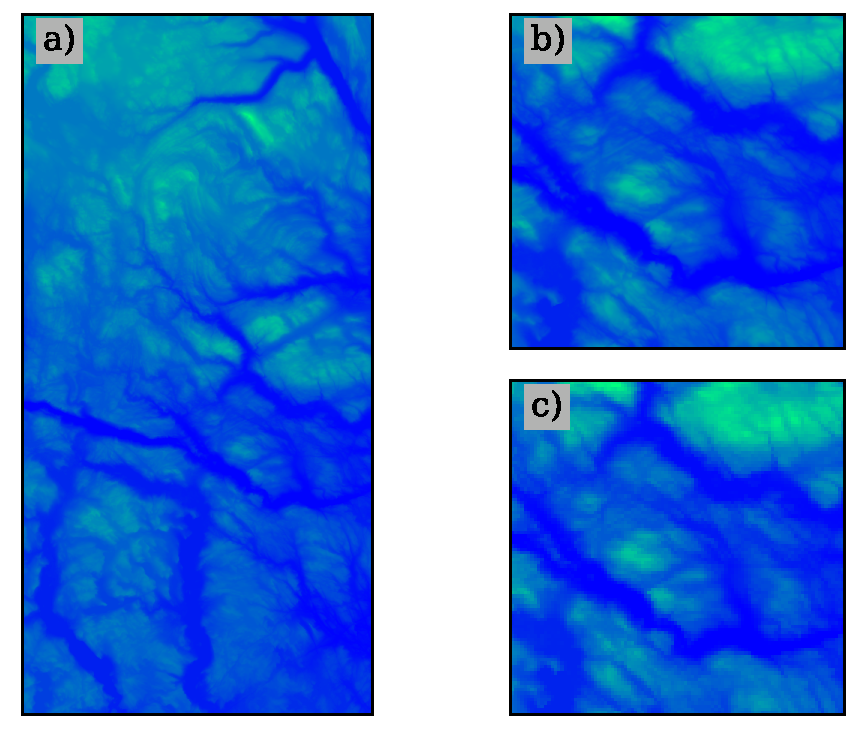
\includegraphics[width = \linewidth]{Figures/terrain_select.pdf}
    \caption{Illustration of the terrain selecting process. Panel a) shows the full terrain dataset. Panel b) Shows the snipped out region of the dataset. Panel c) is a selection of every 10-th datapoint in panel b).}
    \label{fig:terrain_select}
\end{figure}
After selecting the final terrain region, we normalise the data. This is done by finding the maximum and minimum value of the dataset, $z_{max}$ and $z_{min}$, and for every datapoint $z$ in the dataset, performing the following transformation:
\begin{equation}
    z \rightarrow \frac{z - z_{min}}{z_{max} - z_{min}}.
\end{equation}


\section{Results and Discussion}
\label{results}

All the test data is produced by a noisy Franke function, $F (x, y) = f(x, y) + N(x, y, \mu =  0, \sigma = 0.1)$, where $f(x,y)$ is the Franke function in Eq.~\eqref{eq:franke}, and $N$ is randomly distributed noise drawn from the normal distribution with mean $\mu = 0$ and standard deviation $\sigma = 0.1$ at coordinate $(x, y)$.

\subsection{OLS}

The MSE and $R^2$ scores for the OLS regression on the Franke function are shown in Figure~\ref{fig:ols_mse}. We investigate polynomials up to degree $p = 14$ to explore the region where the MSE flattens out and to observe it increasing again as the complexity (\textit{i.e.} polynomial degree) becomes sufficiently large. The MSE decreases with polynomial degree and flattens out. The data was split into a train and test interval, with test size = 0.2. We have also plotted the MSE from the $k$-fold cross validation and bootstrap algorithms, as well as the $R^2$ score for the cross validation. For sufficiently large polynomial degrees, neither of these algorithms are seen to improve the MSE above the value obtained using just the simple split, shown in red with circular markers.

\begin{figure} [h!]
    \centering
    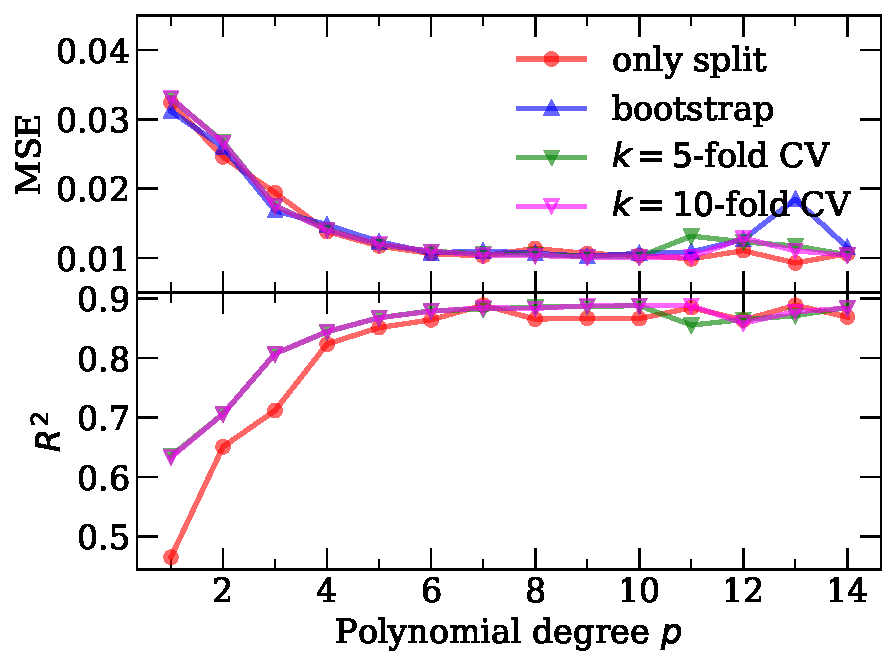
\includegraphics[width = \linewidth]{Figures/ols_stat.pdf}
    \caption{The mean square error (upper panel) and the $R^2$-score (lower panel) produced by OLS regression on a dataset generated by the Franke function. A grid size of $N = 50 \times 50$ was used.}
    \label{fig:ols_mse}
\end{figure}

The bias-variance trade off for OLS regression is studied in Figure~\ref{fig:ols_bivar}. We study two different grid sizes (\textit{i.e.} number of data points) as the difference is quite dramatic. We have employed bootstrap resampling with the number of bootstrap runs $k_B = 100$. Both grid sizes overall feature a low variance and a squared bias almost equal to the MSE. However, for the small grid size, there is a cross over between the bias and the variance for polynomial degree $p = 9$. The variance overtakes the bias and increases dramatically, whereas the bias is decreased. This does not happen for a the larger data point grid, where the variance remains almost at 0 for every polynomial degree studied. 

\begin{figure} [h!]
    \centering
    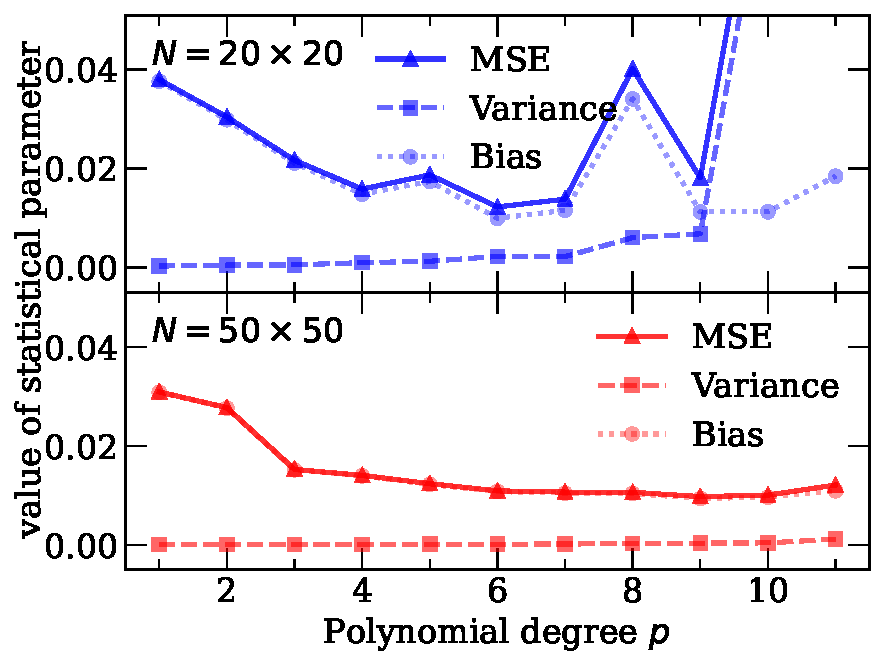
\includegraphics[width = \columnwidth]{Figures/ols_bias_var.pdf}
    \caption{The bias-variance tradeoff studied using the bootstrap algorithm for OLS regression on two different datagrid sets for the Franke function.}
    \label{fig:ols_bivar}
\end{figure}

The low variance we observe for the larger grid size is further supported by Figure~\ref{fig:ols_beta}. Here we study the variance of the OLS regression coefficients $\beta_j$ for the same two grid sizes as in Figure~\ref{fig:ols_bivar}. We have used polynomial degree $p = 5$ to obtain the coefficients. The error bars are taken to be the $\mathrm{Var}(\beta_j)$. As stated earlier, this is proportional to the irreducible error $\sigma^2$, which arises from the noise added to the Franke function, and the diagonal element of the matrix $(\mathbf{X}^T\mathbf{X})^{-1}$.  
\begin{figure} [h!]
    \centering
    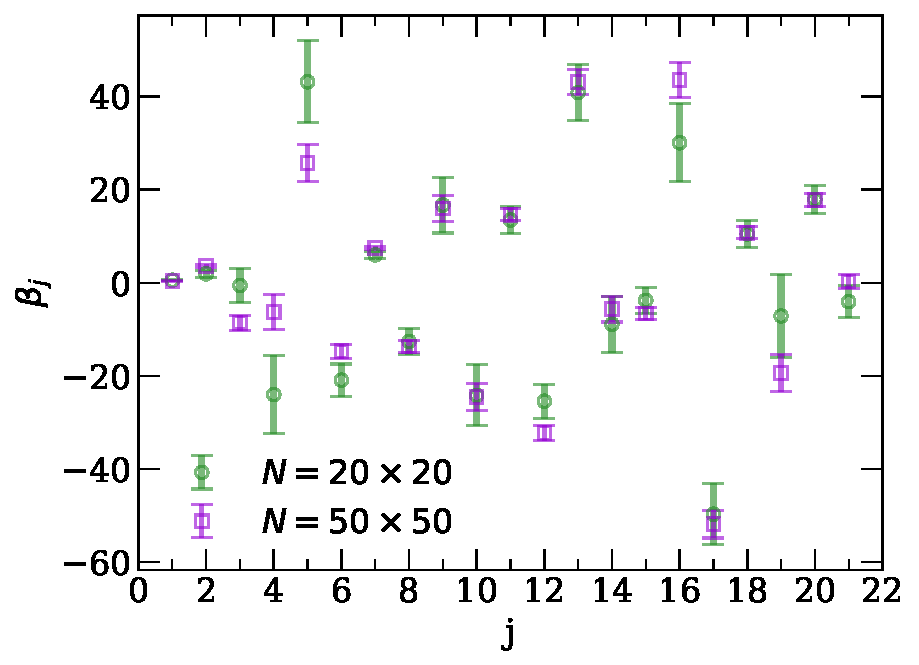
\includegraphics[width = \columnwidth]{Figures/beta_var.pdf}
    \caption{The coefficients $\beta_j$ of the OLS regression vector $\bm{\beta}$ for a polynomial of degree $p = 5$. The coefficients are computed on two different data point grids as indicated by the legend. The error bars are taken to be $\mathrm{Var(\beta_j)}$. Observe that the variance decreases with the number of points.}
    \label{fig:ols_beta}
\end{figure}

\subsection{Ridge}

MSE plots for ridge regression on the Franke function are shown in Figures~\ref{fig:mse_ridge_20} and \ref{fig:mse_rdige_50}. The two figures differ in the grid of $(x,y)$-points used to generate the Franke function, and are the same two studied for OLS. The upper panel of the figures show the MSE using a $k = 5$ fold cross validation resampling, whereas the lower panel uses $k = 10$.

\begin{figure}
    \centering
    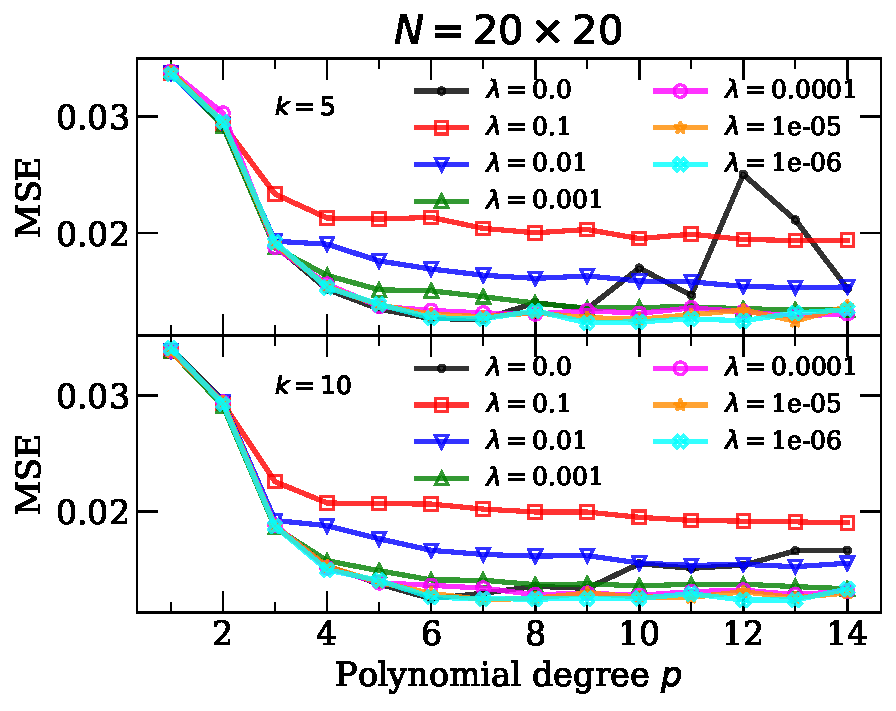
\includegraphics[width = \columnwidth]{Figures/mseRidge_n20.pdf}
    \caption{Mean square error for ridge regression on the Franke function with a gridsize of $(N_x,N_y) = (20, 20)$. The upper panel shows a $k = 5$-fold cross validation, the lower $k = 10$.}
    \label{fig:mse_ridge_20}
\end{figure}

\begin{figure}
    \centering
    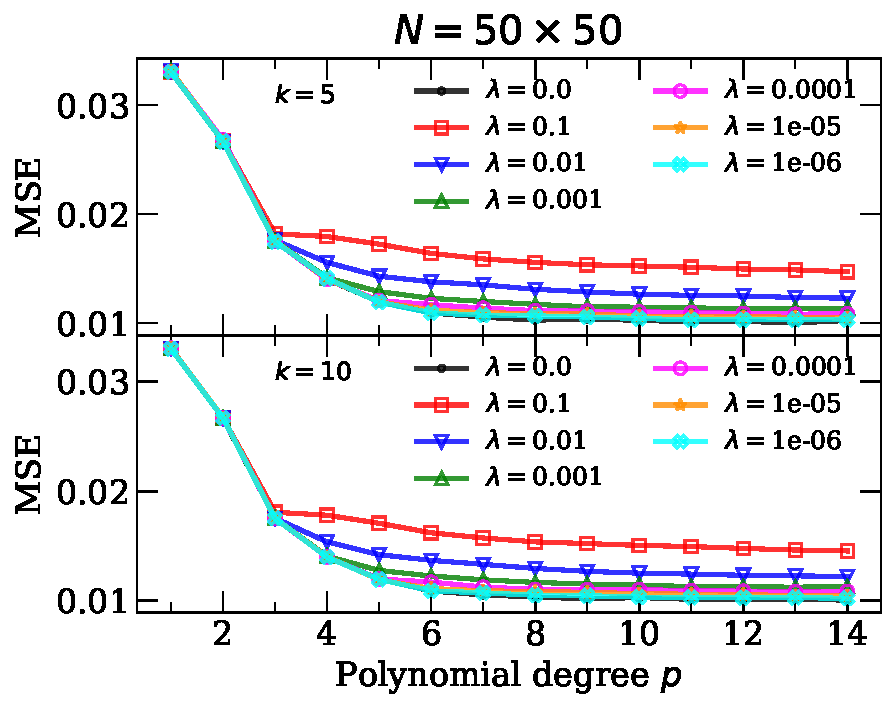
\includegraphics[width = \columnwidth]{Figures/mseRidge_n50.pdf}
    \caption{Mean square error for ridge regression on the Franke function with a gridsize of $(N_x,N_y) = (50, 50)$. The upper panel shows a $k = 5$-fold cross validation, the lower $k = 10$.}
    \label{fig:mse_rdige_50}
\end{figure}

For both grid sizes and both $k$-values the lowest MSE is achieved by $\lambda = 0$, which is equivalent to OLS. For large polynomial degrees, the low-point density OLS MSE starts increasing again above $p = 9$, but for the high-point density grid the OLS case remains the best. Apart from the OLS, the lowest MSE is achieved for the lowest value of $\lambda$ and the highest MSE is obtained for the largest value of $\lambda$. This is unsurprising considering OLS seemingly gives the best result, and a smaller $\lambda$ implies the ridge regression gives results closer to OLS. 

We have also applied the bootstrap algorithm to investigate the bias-variance trade off for ridge regression. The results are shown in Figures~\ref{fig:bivar_rdige_20} and \ref{fig:bivar_ridge_50}. We investigated two of the $\lambda$ values used in computing the MSE; the one giving the best results and the one giving the worst. The worst (\textit{i.e.} largest) lambda is shown in the upper panels and the best in the lower. The two figures again represent the two different grid sizes we are investigating. As we saw with for OLS regression, the smaller grid in Figure~\ref{fig:bivar_rdige_20}, especially for the "good" $\lambda$ in the lower panel, shows that the variance becomes finite for large polynomial degrees, decreasing the bias. 

\begin{figure}
    \centering
    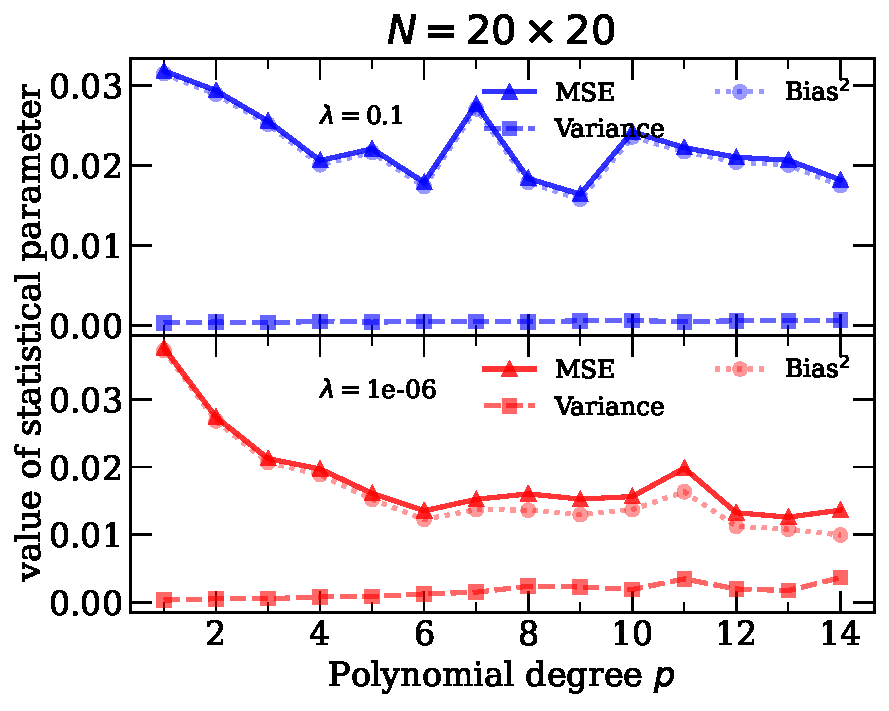
\includegraphics[width = \columnwidth]{Figures/biasvar_ridge_n20.pdf}
    \caption{The bias-variance trade off investigated using the bootstrap algorithm with $k_B = 100$ and ridge regression with $\lambda$ as indicated in the panels. Data generated by the Franke function on a grid of points $(N_x, N_y) = (20,20)$.}
    \label{fig:bivar_rdige_20}
\end{figure}

\begin{figure}
    \centering
    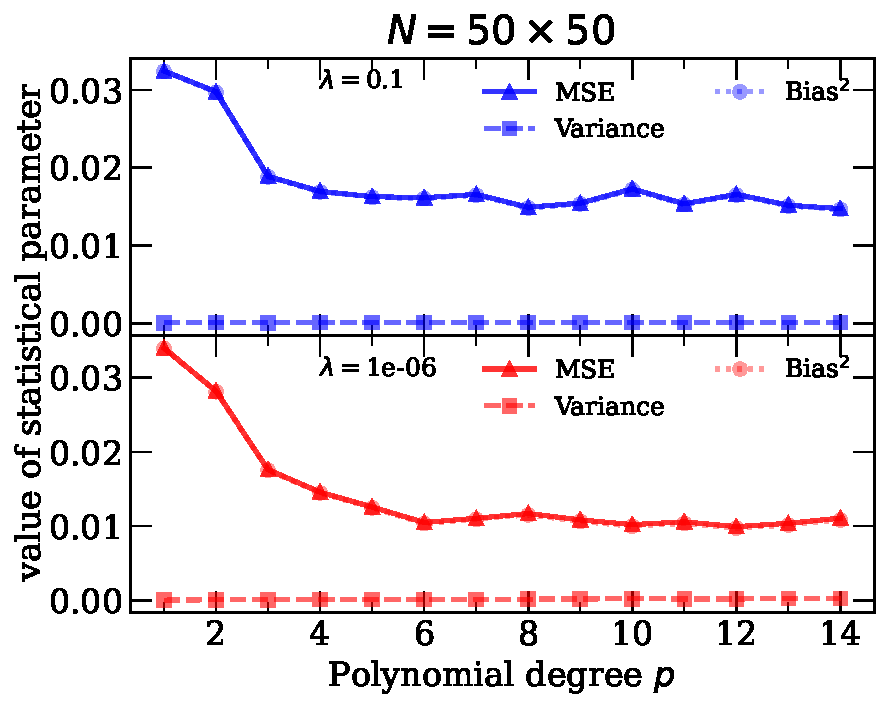
\includegraphics[width = \columnwidth]{Figures/biasvar_ridge_n50.pdf}
    \caption{The bias-variance trade off investigated using the bootstrap algorithm with $k_B = 100$ and ridge regression with $\lambda$ as indicated in the panels. Data generated by the Franke function on a grid of points $(N_x, N_y) = (50,50)$.}
    \label{fig:bivar_ridge_50}
\end{figure}

\subsection{Lasso}

MSE plots of lasso regression on the Franke function are shown in Figures~\ref{fig:mse_lasso_20} and \ref{fig:mse_lasso_50}. Both are generated using $k$-fold cross validation, with $k = 5$ in the upper panel and $k = 10$ in the lower panel. The two figures, as before, show the MSE for the two $(x,y)$ grids we have studied throughout this text. As with ridge regression, the MSE improves with smaller values of $\lambda$. The lasso-algorithm is not well defined for $\lambda = 0$ (OLS) and this result is therefore not included in the figures. Nevertheless it is evident when compared to the results obtained for ridge and OLS regression that lasso regression gives a larger MSE than the methods studied earlier. 

\begin{figure}
    \centering
    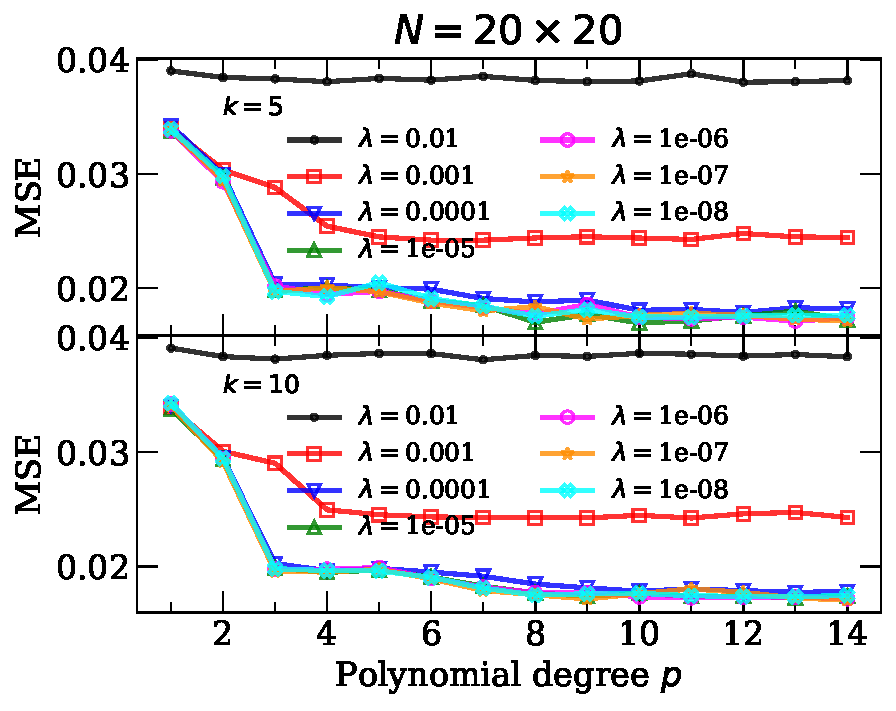
\includegraphics[width = \columnwidth]{Figures/mseLasso_n20.pdf}
    \caption{Mean square error for lasso regression on the Franke function with a gridsize of $(N_x,N_y) = (20, 20)$. The upper panel shows a $k = 5$-fold cross validation, the lower $k = 10$.}
    \label{fig:mse_lasso_20}
\end{figure}

\begin{figure}
    \centering
    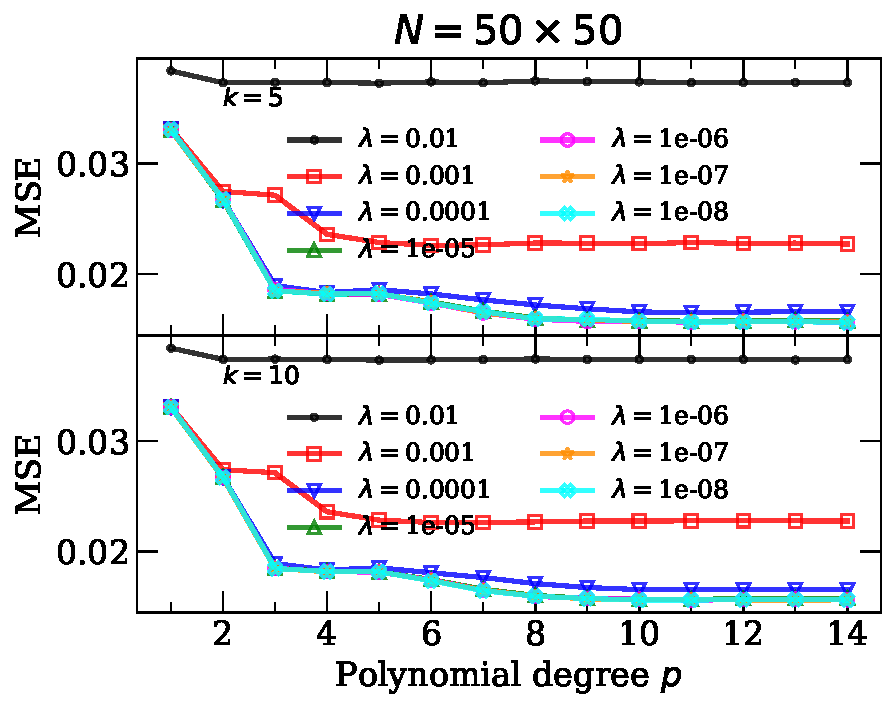
\includegraphics[width = \columnwidth]{Figures/mseLasso_n50.pdf}
    \caption{Mean square error for lasso regression on the Franke function with a gridsize of $(N_x,N_y) = (50, 50)$. The upper panel shows a $k = 5$-fold cross validation, the lower $k = 10$.}
    \label{fig:mse_lasso_50}
\end{figure}

We have also looked at the bias-variance trade off using lasso regression. The results are presented in Figure~\ref{fig:bivar_lasso}. This time we only looked at the low point density grid,  $(N_x,N_y) = (20, 20)$, as the results were practically identical between the two, and not much different from the high point density grid we studied using ridge regression in Figure~\ref{fig:bivar_ridge_50}.  
\begin{figure} [h!]
    \centering
    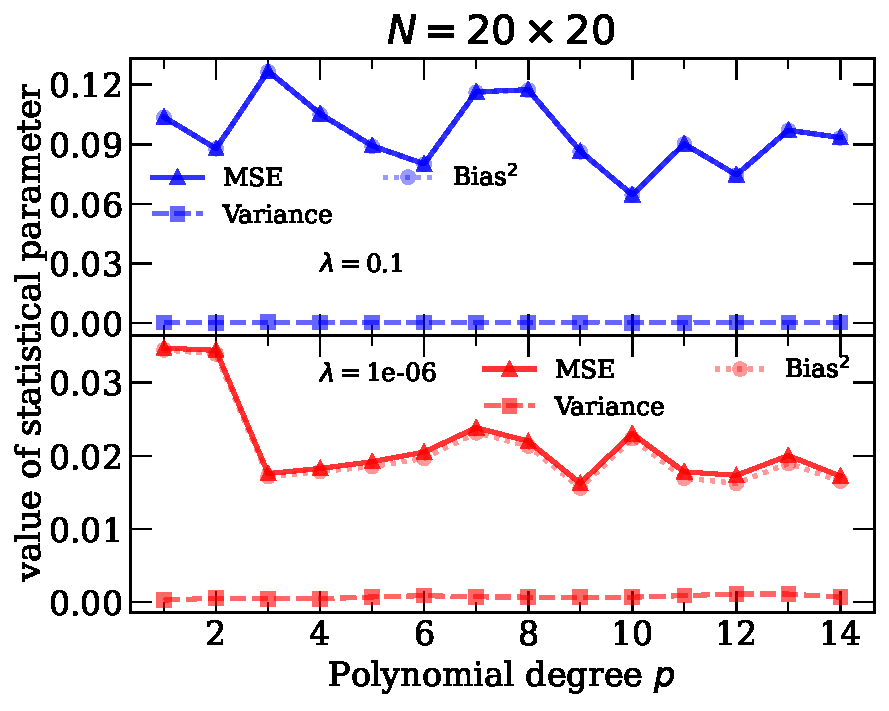
\includegraphics[width = \columnwidth]{Figures/biasvar_lasso_n20.pdf}
    \caption{The bias-variance trade off investigated using the bootstrap algorithm with $k_B = 100$ and lasso regression with $\lambda$ as indicated in the panels. Data generated by the Franke function on a grid of points $(N_x, N_y) = (20,20)$.}
    \label{fig:bivar_lasso}
\end{figure}
Again we chose to study a high and low value of $\lambda$. For the high value of $\lambda$, which gives the worst MSE, the variance remains approximately zero for each studied polynomial degree, whereas the square bias closely follows the MSE. For the low value of $\lambda$ we obtain a finite, but small, variance implying that the square bias drops below the MSE. 

\subsection{Intermezzo}
Before proceeding with evaluating our model on terrain data we summarise and discuss what we have learned from applying the regression methods to the Franke function. 
The first observation is that OLS gives the smallest MSE overall, and that for large enough polynomial degree, the MSE flattens out. The same is true for the $R^2$-score, which flattens out and approaches unity. The Franke function is a sum of exponentials, which can be Taylor expanded as a series of powers in $x$ and $y$. Thus it is no surprise that the MSE decreases with increasing polynomial degree, as we can more accurately describe each power in the Taylor series with increasing polynomial degree. Furthermore, the $n$-th term in the Taylor series is proportional to $1/n!$, implying that they become less and less important. This is what is reflected when the MSE flattens out with increasing polynomial degree. There is a caveat however. As explained in \textit{e.g.} Ref.~\cite{Hastie}, with larger polynomial degree we run the risk of overfitting. When this happens, the polynomials will start fitting the noise present in the data as well, not just the Franke function. This increases the variance and lowers the bias. This effect is present in the upper panel of Figure~\ref{fig:ols_bivar}. However, as we observe, increasing the number of data points can mitigate the overfitting effect for a given polynomial degree. This is evident both from comparing the upper and lower panels of Figure~\ref{fig:ols_bivar}, and from the variance of the regression coefficients $\beta_j$ in Figure~\ref{fig:ols_beta}. When moving on from OLS to ridge and lasso regression the overfitting issue is less apparent. In all cases where we tested the bias-variance trade off for ridge and lasso regression, the variance remained close to zero. Summarised we therefore see that OLS has given us the lowest MSE, and when remaining conscious about polynomial degrees and the number of datapoints in our grid, an increasing variance has not given us issues with increasing the MSE.

\subsection{Terrain Data}

We now present the MSE of OLS, ridge and lasso regression performed on the terrain data. We performed two sets of OLS regression; one set on unnormalised terrain data and one set on normalised terrain data. For all instances we performed both 5-fold and 10-fold cross validation. 

OLS on unnormalised and normalised terrain data is presented in Figures~\ref{fig:ols_terrain_non} and \ref{fig:ols_terrain}, respectively. Both instances give the lowest MSE for polynomial degree $p = 10$, for both 5- and 10-fold corss validation. Beyond $p = 10$, the MSE blows up. likely due to the previously discussed bias variance trade off. It is also worth nothing that the shape of the MSE in both figures is identical. The scale on the ordinate differs, but that is due to the normalisation. The MSE itself is not normalised by the scale of the data. 

\begin{figure}
    \centering
    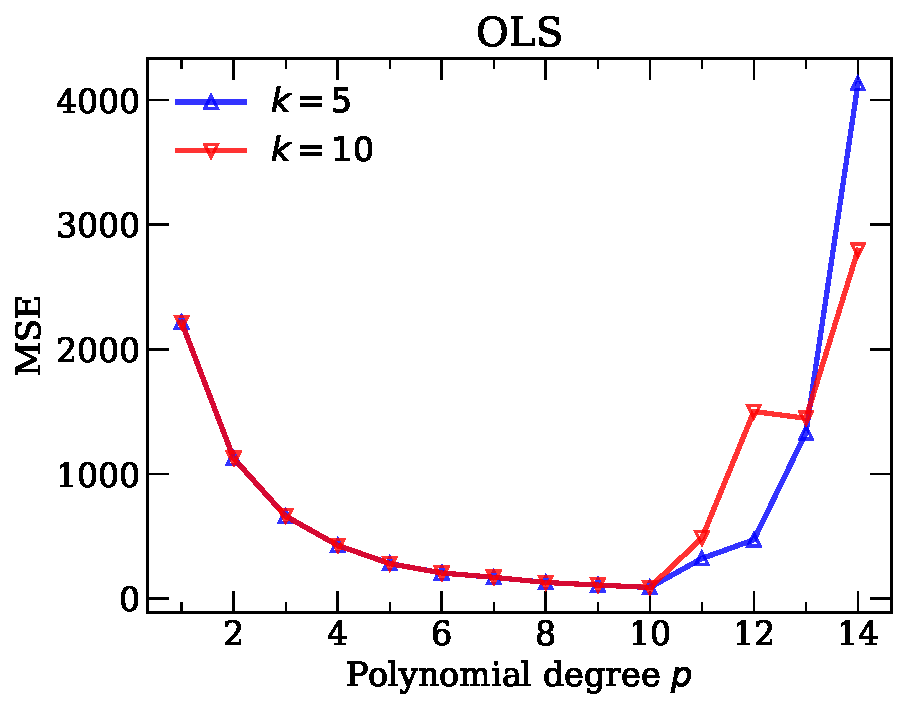
\includegraphics[width = \columnwidth]{Figures/terrain_unscaled_ols.pdf}
    \caption{OLS regression on unnormalised terrain data using both 5- and 10-fold cross validation, as indicated in the legend. }
    \label{fig:ols_terrain_non}
\end{figure}

\begin{figure} [h!]
    \centering
    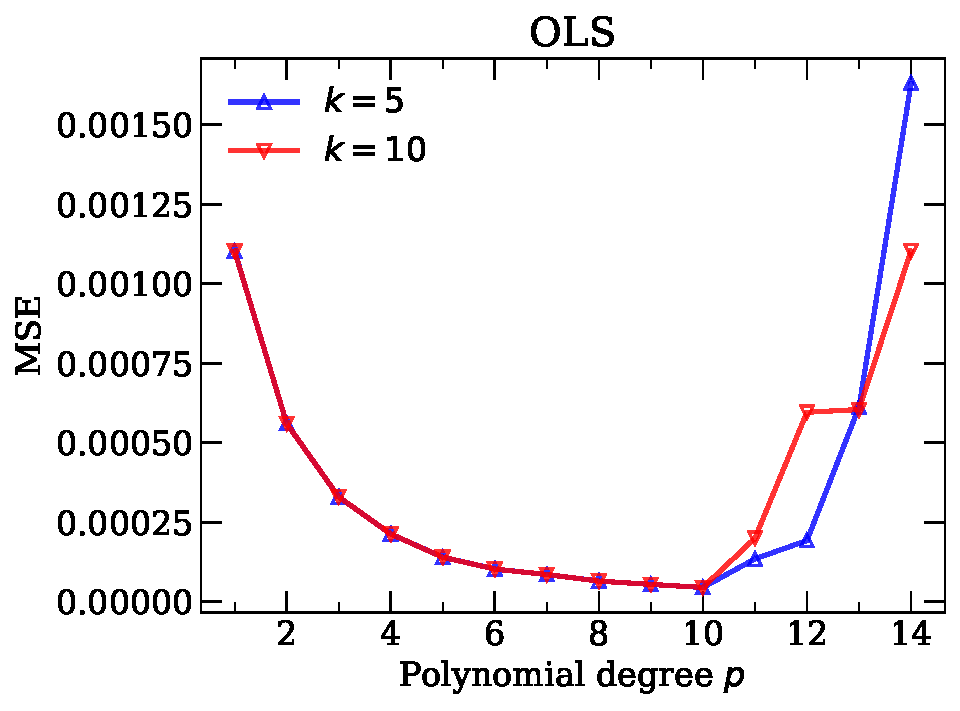
\includegraphics[width = \columnwidth]{Figures/terrain_scaled_ols.pdf}
    \caption{OLS regression on normalised terrain data using both 5- and 10-fold cross validation, as indicated in the legend.}
    \label{fig:ols_terrain}
\end{figure}

MSE for ridge and lasso regression is shown in Figures~\ref{fig:ridge_terrain} and \ref{fig:lasso_terrain} respectively. The upper panels show $k = 5$-fold cross validation and the lower panels show $k = 10$-fold cross validation. In both instances, as for the Franke function, a $\lambda$ closer to zero gives a lower MSE. We went to a higher polynomial degree to investigate if we could see the MSE flatten out, but we have not yet reached that region for $p = 18$ for the $\lambda$-values closest to zero. 

\begin{figure}
    \centering
    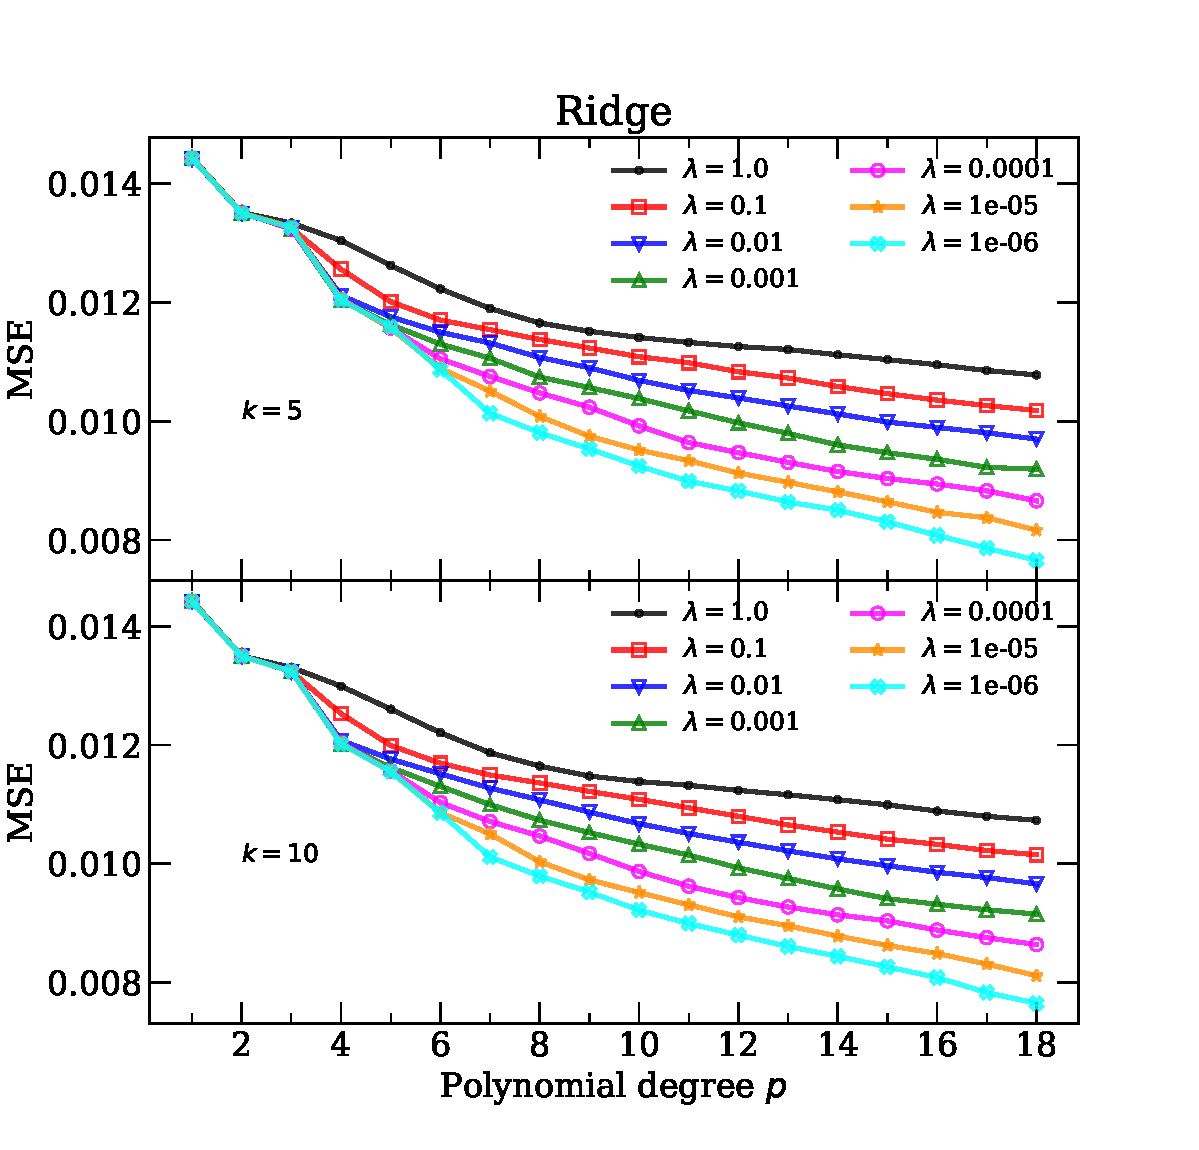
\includegraphics[width = \columnwidth]{Figures/terrain_scaled_ridge.pdf}
    \caption{Ridge regression on normalised terrain data. 5-fold cross validation in the upper panel, 10-fold cross validation in the lower panel. Range of $\lambda$ indicated in the figure legend.  }
    \label{fig:ridge_terrain}
\end{figure}

\begin{figure}
    \centering
    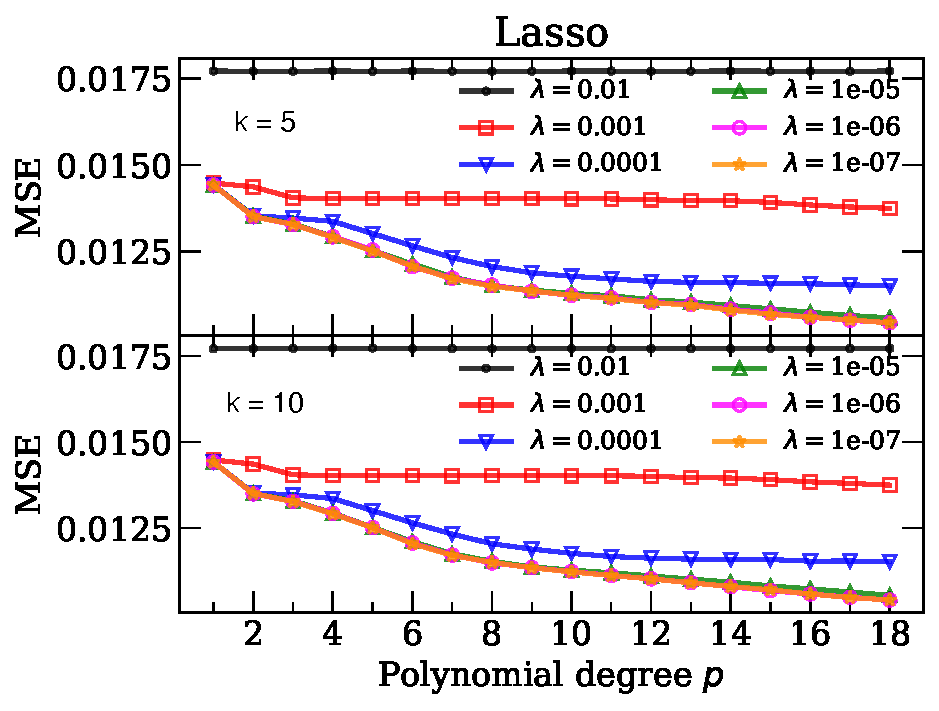
\includegraphics[width = \columnwidth]{Figures/terrain_scaled_lasso.pdf}
    \caption{Lasso regression on normalised terrain data. 5-fold cross validation in the upper panel, 10-fold cross validation in the lower panel. Range of $\lambda$ indicated in the figure legend.  }
    \label{fig:lasso_terrain}
\end{figure}

As we observed when examining the regression results for the Franke function, the same trends are present in the regression results for the terrain data. The MSE for both ridge and lasso regression is much larger than the MSE we obtain from OLS. Furthermore, OLS obtains an MSE minimum at $p = 9$, whereas ridge and lasso still are approaching their minima for $p = 18$. Extrapolating the results we obtained for the Franke function, we do not expect the minima of neither ridge or lasso regression to give a smaller MSE than for OLS. This is further supported by the fact that the MSE of ridge and lasso regression is smaller for smaller $\lambda$. We therefore expect the minima of the MSE of both ridge and lasso to be at $\lambda = 0$; \textit{i.e.} OLS regession. 
There is somewhat of a surprise associated with the fact that we observe an increasing MSE with OLS on the terrain data for large $p$. Intuitively, one would think that the terrain data is so complex that it was hard to generate overfitting. This overfitting is not reproduced by ridge and lasso regression. Separate runs, not shown herein, indicate that the overfitting issue is only an issue for $p = 13$ and $p = 14$. This could imply that we have implemented some sort of systematic error in our code that fails for polynomials of these degrees. 
The overall takeaway from both studying the Franke function and the terrain data is that OLS performs best, and that we only once saw a bias-variance crossover. The latter implies that the variance has remained small for all methods, in turn rendering the advantages of ridge and lasso regression over OLS small. This is reflected in the fact that lasso and ridge regression performs best for small $\lambda$ -- when they are close to true OLS. The likely cause is that the data is complex enough to prevent overfitting, even at large polynomial degrees, rendering the OLS method superior.

\section{Conclusion}

We have performed compared three different methods of linear regression (OLS, ridge and lasso) on two sets of data; one set generated by the analytic Franke function, and one set of real world terrain data. Analysing the Franke function, we observed the bias-variance crossover using OLS and we found that OLS gave the lowest MSE of the three methods. Furthermore, we observed that increasing the number of datapoints used to generate the Franke function reduced the variance and prevented overfitting. The observations we made on the Franke function were consistent with the ones we made analysing the terrain data, where we again find that OLS gives the best MSE. We understand this in terms of the large complexity of the data. This complexity lead to no overfitting of the data, even for large polynomial degree, which in turn cancelled the advantages of ridge and lasso regression over OLS. 

%Bibliography
\begin{thebibliography}{4}


\bibitem{Hastie}
T.~Hastie, R.~Tibshirani, and J.~Friedman.
\textit{The Elements of Statistical Learning}.
Springer, New York, 2009.

\bibitem{Franke}
R. Franke
\textit{A Critical Comparison of Some Methods for Interpolation of Scattered Data}
Naval Postgraduate School, California, 1979.

\bibitem{James}
G.~James, D.~Witten, T.~Hastie, and R.~Tibshirani.
\textit{An Introduction to Statistical Learning}.
Springer, New York, 2017.

\bibitem{Hoerl}
A.~E.~Hoerl, R.~W.~Rennard, (1970). Ridge Regression: Biased Estimation for Nonorthogonal Problems. \textit{Technometrics}, 12(1), 55–67. 

\end{thebibliography}


\end{document}